\documentclass[a4paper, 12pt]{report}
\usepackage{cs_thesis}
\usepackage[pdftex]{graphicx}
\usepackage[utf8]{inputenc}
\usepackage{amsmath}
\usepackage{url}
\usepackage{biblatex}
\usepackage{listings}
\usepackage{color}

\renewcommand{\UrlFont}{\small\tt}

\title{The iCub Humanoid Robot}
\author{Semih Onay}
\program{Computer Science}
\supervisor{Associated Professor Elena Battini Sönmez}


\begin{document}
\pagenumbering{roman}
\makecstitle

\tableofcontents
\listoffigures
\listoftables

\begin{symabbreviations}
\sym{\textbf{YARP}}{Yet Another Robot Platform}
\sym{}{} 
\sym{DA}{Description of abbreviation}
\end{symabbreviations}

\chapter*{ABSTRACT}
Robot are evolving to the dead ends. Software and hardware they produce, 
disappearing without trace afterwards. Here, exploring how to make our 
projects stable and long-lasting, without yielding our ability to 
constantly change our sensors, actuators, processors, and networks.
We advance on two fronts, software and hardware. For some time, we have been 
developing and using the YARP robot software architecture, which helps 
organize communication between sensors, processors, and actuators so that loose 
coupling is encouraged, making gradual system evolution much easier. YARP 
includes a model of communication that is transport-neutral, so that data flow 
is decoupled from the details of the underlying networks and protocols in use. 
Importantly for the long term, YARP is designed to play well with other 
architectures.
\begin{figure}[h!]
\centering
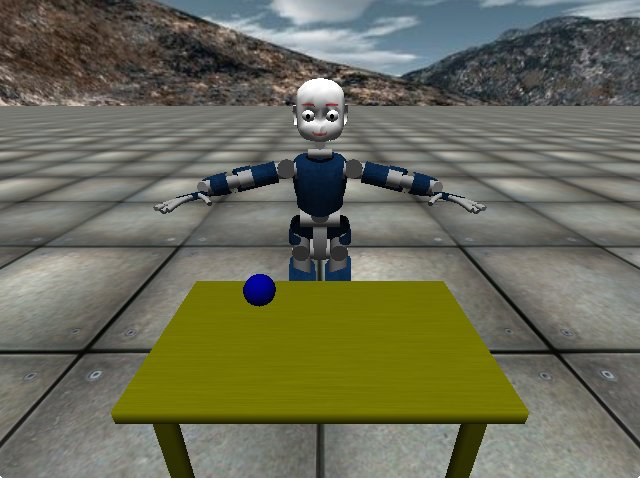
\includegraphics[width=0.8\linewidth]{sim}
\caption{}
\label{fig:sim}
\end{figure}
 Device drivers written for YARP can be ripped out and used 
without any “middleware.” On the network, basic interoperation is possible with 
a few lines of code in any language with a socket library, and maximally 
efficient interoperation can be achieved by following documented protocols. 
These features are not normally the first things that end-users look for when 
starting a project, but they are crucial for longevity.
We emphasize the strategic utility of the Free Software social contract to 
soft- ware development for small communities with idiosyncratic requirements. 
We also work to expand our community by releasing the design of our ICub 
humanoid under a free and open license, and funding development using this 
platform.

\chapter*{ÖZET}


\chapter{INTRODUCTION}

The iCub is a humanoid robot developed at Istituto Italiano di Tecnologia (IIT) 
as part of the European project RobotCub and later adopted by more than 20 
laboratories arround the world. It has 53 motors that can move the head, arms 
and hands, midriff, and legs.It can see and hear, it has the sense of 
proprioception (body 
configuration) and movement (using accelerometers and gyroscopes).
It’s designed to aid studies of human cognition and artificial 
intelligence. Project members developed computer simulator to experiment new 
techniques.
\par Computer simulations are getting important in area robotics 
area.Simulations may not provide real complexity of the physical world and not 
reliable as real dynamics. The simulator of iCub is an easy way to test new 
algorithms and methods instead of dealing with complex configuration of iCub 
hardware. The simulator is designed to be accurate as real world psychics and 
dynamics. Development is based on directly from first prototype of simulation 
environment Webots[1]. Webots was expensive and had limited access to source 
code which made hard to modify source code in order to add some properties.Then 
iCub simulation created.Simulation environment uses 
\cite{ODE} to simulate 
body movement and collision detection algorithms to measure psychical 
interaction with the world.ODE is used in wide range of projects like Gazebo 
project. ODE is an open source physics engine for authoring tools, computer 
games,etc.It uses OpenGL renderer and it has some disadvantages due to 
limitation of OpenGL engine computation efficiency on complex structures.iCub 
simulation uses OpenGL directly via SDL which helps to render complex robot 
movements and com- putation efficient simulation observations. Simulator is 
free and available to anyone who interested in robotics and learning about 
basics of robotics.


\chapter{LITERATURE REVIEW}

Development of simulator is described by abstraction of parts to handle complex 
instructions more precisely and efficient. Some other external software 
libraries are used to reduce required time to animate given parts of robots 
body from parameters. Abstractions made it easy to implement new 
methods,algorithms into a simulation environment. Understanding of these 
libraries are the key of creating new interfaces and methods to robot in 
virtual world.
Action primitives are pre-defined inside a simulation environment to extend ca- 
pability of creating new interfaces to virtual simulation world and can be 
changed or taught as different languages which helps to extend knowledge about 
languages.

\chapter{METHODOLOGY}

\subsection{The YARP Arcitechture}
The computer simulation model of the iCub robot.The simulator allows to 
create realistic scenarios in where robot can interact with a virtual world and 
physical limitations and interactions that occur between the virtual world is 
simulated using open source library which is ODE (Open Dynamics Engine) to 
provide accurate simulation of body dynamics.

\begin{figure}[h!]
\centering
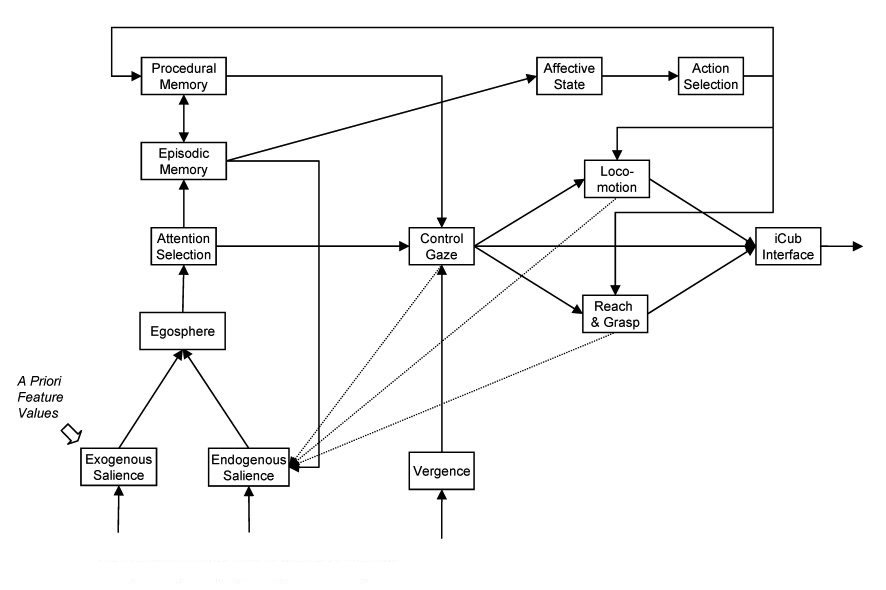
\includegraphics[width=1.0\linewidth]{cognitive_architecture}
\caption{}
\label{fig:cognitive_architecture}
\end{figure}

Top of \cite{YARP}. It is a set of open source 
libraries that supports modularity by using abstraction method in softwares to 
handle common difficulties in robotics area which are know as modularity 
algorithms and hardware in- terfaces and OS platforms.To deal with OS spesific 
builds,requires to use cross-platform build tools such as \cite{Cmake} and 
\cite{ACE}.
YARP is providing platform independence.First abstraction can be described as a 
protocols.Main YARP protocol manages inter-process communications in operating 
systems.It can deliver process messages of any size across the network by using 
different protocols.

Second abstraction is about hardware communications.The method is to define 
interface for class of devices to fold native coded APIs.Changes in hardwares 
requires changes in API calls via linking suitable libraries to encapsulate 
hardware dependency problems. These two abstraction combined to use remote 
device drives where that can be accessed across the network like a parallel 
processing.

The purpose of YARP ports are to move data from threads to threads over the 
processes.Flow of the data can be configured and observed from command-line at 
real- time.Port can receive or send data from any other port.Connections 
between ports can be modified easily with using different protocols such as 
TCP(Transmission Control Protocol) and UDP(User Datagram Protocol).The choice 
of protocol is depends on quality of message transmission or response 
time.Using TCP is for reliability and UDP is for speed with effect on 
unreliable transmissions.
\begin{figure}[h!]
  \centering
  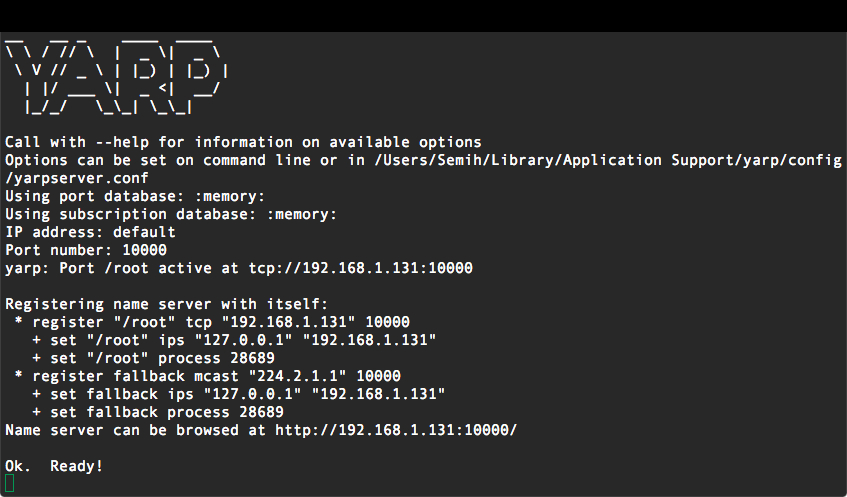
\includegraphics[width=0.8\linewidth]{yarp}
  \caption{}
  \label{fig:yarp}
\end{figure}
\subsection{Mechanics of iCub}

2.1 Mechanics
The kinematic specifications of the body of the iCub including the definition 
of the number of DOF and their actual locations as well as the actual size of 
the limbs and torso were based on ergonomic data and x-ray images.
The possibility of achieving certain motor tasks is favored by a suitable 
kinematics and, in particular, this translates into the determination of the 
range of movement and the number of controllable joints (where clearly 
replicating the human body in detail is impossible with current technology). 
Kinematics is also influenced by the overall size of the robot which was 
imposed a priori. The size is that of a 3.5 years old child (approximately 
100cm high). This size can be achieved with current technology. QRIO1 is an 
example of a robot of an even smaller size although with less degrees of 
freedom. In particular, our task specifications, especially manipulation, 
require at least the same


\begin{figure}[h!]
\centering
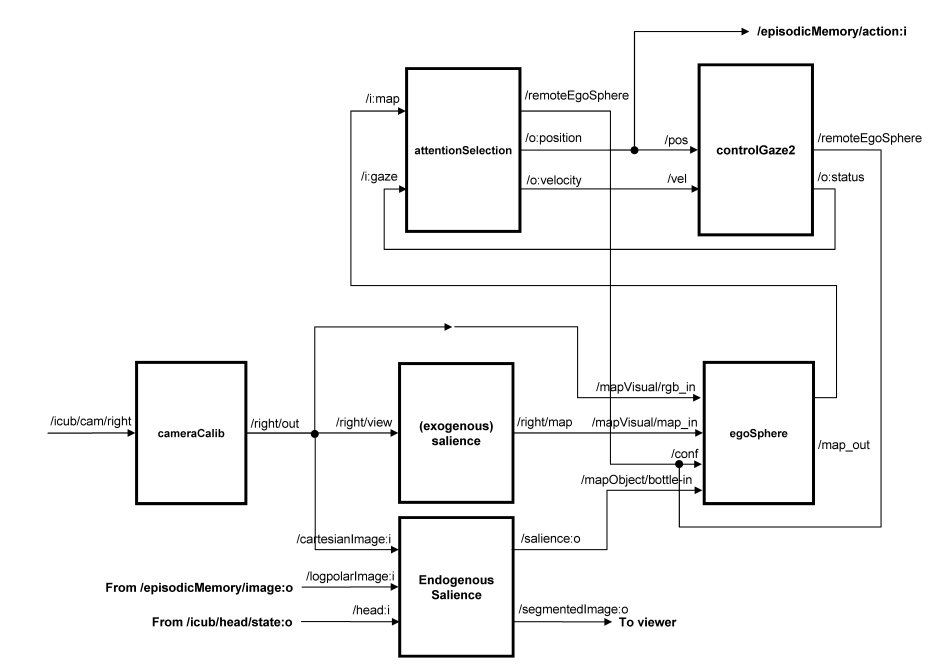
\includegraphics[width=0.9\linewidth]{cognitive_architecture_A}
\caption{}
\label{fig:cognitive_architecture_A}
\end{figure}


\chapter{RESULTS}

\lstset{language=C++,
  basicstyle=\ttfamily,
  keywordstyle=\color{blue}\ttfamily,
  stringstyle=\color{red}\ttfamily,
  commentstyle=\color{green}\ttfamily,
  morecomment=[l][\color{magenta}]{\#}
}

\lstset{language=C++,
 keywordstyle=\color{blue},
 stringstyle=\color{red},
 commentstyle=\color{green},
 morecomment=[l][\color{magenta}]{\#}
}

\begin{lstlisting}

public:objectMoverThread(ResourceFinder &_rf) : rf(_rf) {
        virtual bool loadParams() {
  
  name = rf.check("name",Value("objectMover")).asString().c_str();
  neckTT = rf.check("necktt",Value(2.0)).asDouble();
  eyeTT = rf.check("eyett",Value(1.2)).asDouble();
  trajTime = rf.check("trajtime",Value(4.0),"Solver trajectory 
  time").asDouble();
  maxPitch = rf.check("maxpitch",Value(30.0),"Torso max pitch").asDouble();
  
  //get which arm to use. default to left if they didnt pass in left or right
  armname = rf.check("arm", Value("left"),"arm name").asString().c_str();
    if (armname == "right") {
      armInUse = true;
    }
    else {
      armInUse = false;
    }
  
  //get which robot target to use
  robotname = rf.check("robot", Value("icub"),"robot name").asString().c_str();
  
}
  \end{lstlisting}

\chapter{TITLE OF THE FIRST APPENDIX}

\appendix

\begin{thebibliography}{9}
\bibitem{Webots} 
Webots: robot simulation software
\\\texttt{https://www.cyberbotics.com}

\bibitem{ODE} 
ODE: Open Dynamics Engine
\\\texttt{http://www.ode.org}

\bibitem{YARP} 
YARP: Yet Another Robot Platform 
\\\texttt{http://wiki.icub.org/yarp/}

\bibitem{CMake} 
CMake: Cross-Platform Open Source Build System 
\\\texttt{http://www.cmake.org}

\bibitem{ACE} 
ACE: The ADAPTIVE Communication Environment
\\\texttt{http://www.cs.wustl.edu/~schmidt/ACE.html}

\bibitem{iCub} 
iCub: An Open Source Cognitive Humanoid Robotic Platform
\\\texttt{http://www.icub.org}

\end{thebibliography}

\end{document}